%%% LaTeX Template: Article/Thesis/etc. with colored headings and special fonts
%%%
%%% Source: http://www.howtotex.com/
%%% Feel free to distribute this template, but please keep to referal to http://www.howtotex.com/ here.
%%% February 2011
%%%
%%% Modified May 2018 by CDM

%%%  Preamble
\documentclass[11pt,letterpaper]{article}
\usepackage[margin=1.0in]{geometry}
\usepackage[T1]{fontenc}
\usepackage[bitstream-charter]{mathdesign}
\usepackage[latin1]{inputenc}					
\usepackage{amsmath}						
\usepackage{xcolor}
\usepackage{cite}
\usepackage{hyphenat}
\usepackage{graphicx}
\usepackage{float}
\usepackage{subfigure}
\usepackage{sectsty}
\usepackage[compact]{titlesec} 
\usepackage[tablegrid]{vhistory}
\allsectionsfont{\color{accentcolor}\scshape\selectfont}

%%% Definitions
\definecolor{accentcolor}{rgb}{0.0,0.0,0.5} 
\newcommand{\teamname}{UTA STeam}
\newcommand{\productname}{Groco}
\newcommand{\coursename}{CSE 4316: Senior Design I}
\newcommand{\semester}{Spring 2018}
\newcommand{\docname}{System Requirements Specification}
\newcommand{\department}{Department of Computer Science \& Engineering}
\newcommand{\university}{The University of Texas at Arlington}
\newcommand{\authors}{Patrick Faulkner \\ Hozefa Tankiwala \\ Andrew Hands \\ Kiran Karki \\ Uyen Do}

%%% Headers and footers
\usepackage{fancyhdr}
	\pagestyle{fancy}						% Enabling the custom headers/footers
\usepackage{lastpage}	
	% Header (empty)
	\lhead{}
	\chead{}
	\rhead{}
	% Footer
	\lfoot{\footnotesize \teamname \ - \semester}
	\cfoot{}
	\rfoot{\footnotesize page \thepage\ of \pageref{LastPage}}	% "Page 1 of 2"
	\renewcommand{\headrulewidth}{0.0pt}
	\renewcommand{\footrulewidth}{0.4pt}

%%% Change the abstract environment
\usepackage[runin]{abstract}			% runin option for a run-in title
%\setlength\absleftindent{30pt}			% left margin
%\setlength\absrightindent{30pt}		% right margin
\abslabeldelim{\quad}	
\setlength{\abstitleskip}{-10pt}
\renewcommand{\abstractname}{}
\renewcommand{\abstracttextfont}{\color{accentcolor} \small \slshape}	% slanted text

%%% Start of the document
\begin{document}

%%% Cover sheet
{\centering \huge \color{accentcolor} \sc \textbf{\department \\ \university} \par}
\vspace{1 in}
{\centering \huge \color{accentcolor} \sc \textbf{\docname \\ \coursename \\ \semester} \par}
\vspace{0.5 in}
\begin{figure}[h!]
	\centering
   	
\includegraphics[width=0.3\textwidth]{images/whiteTeamLogo.png}
\end{figure}
\vspace{0.5 in}
{\centering \huge \color{accentcolor} \sc \textbf{\teamname \\ \productname} \par}
\vspace{0.5 in}
{\centering \large \sc \textbf{\authors} \par}
\newpage


%\vspace{1 in}
%\centerline{January 13th, 2012}
%\newpage

%%% Revision History
\begin{versionhistory}
  	\vhEntry{0.1}{10.07.2021}{PF}{document creation}
  	\vhEntry{0.2}{10.15.2021}{PF|HT|AH|KK|UD}{first draft}
  	\vhEntry{0.3}{10.12.2015}{PF|HT|AH|KK|UD}{complete draft}
  %	\vhEntry{1.0}{10.20.2015}{AT|GH|CB}{official release}
  %	\vhEntry{1.1}{10.31.2015}{AL}{added customer change requests}
\end{versionhistory}
\newpage

%%% Table of contents
\setcounter{tocdepth}{3}
\tableofcontents
\newpage

%%% List of figures and tables (optional)
\listoffigures
%\listoftables
\newpage

\section{Product Concept}
This section describes the purpose, use and intended user audience for the Groco product. Groco is a grocery shopping application that is compatible with iOS, Android, and web. The user of Groco will be able to search for the grocery items and based on the user's preference such as locations and brands, the system will suggest the best places to shop these items with the lowest prices and fastest route. The system also allow user to search for recipes, add their own recipes and meal plans into their shopping list to perform the optimization and navigation route. 

\subsection{Purpose and Use}
The purpose of this product is to help the users save money and time shopping for groceries as well as providing the convenience in planing their meals. The product provide the optimal suggestion based on the database and is not responsible for the accuracy or changes regarding prices and discounts at the actual stores.  

\subsection{Intended Audience}
The application is an web application and users can access the application from multiple devices. The product is made available publicly and free of charge. The product contain no objectionable material; therefore it is suitable for general grocery shoppers at all ages.

\begin{figure}[h!]
	\centering
   	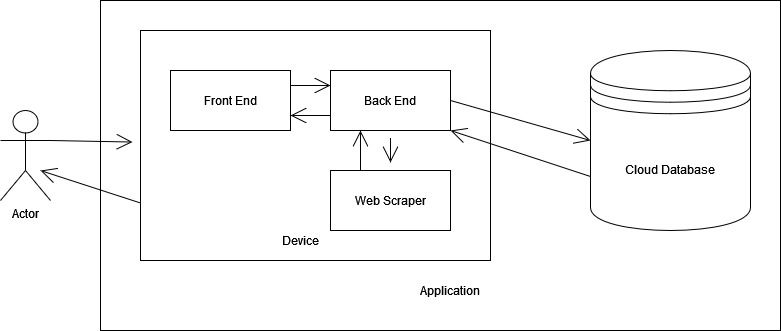
\includegraphics[width=1\textwidth]{images/system_diagram.jpg}
    \caption{High level overview of the system}
\end{figure}

\newpage
\section{Product Description}
Groco is a shopping application that provides the optimal suggestion to shop for groceries. The optimization is based on the user's preferences such as brands, prices, and distance. Groco includes five main components: item search, recipes search, adding recipes, adding meal plan, and navigation.

\subsection{Features \& Functions}
The product suggests the optimal grocery items based on the user's preference. The product consists of five main components:
\begin{itemize}
    \item Atomic item search: A user can search for each item to check its availability and prices.
    \item Recipes search: A user can search for a specific recipe and add it to a shopping list.
    \item Adding customized recipes: A user can add his or her recipes for later use or share with other users.
    \item Adding meal plans: A user can multiple recipes to create meal plans. The product will aggregate all items and amounts for shopping.
    \item Store navigation: A user can click on the map link to navigate to stores.
\end{itemize}
The product provides the optimal suggestion based on the database and is not responsible for the accuracy or changes regarding prices and discounts at the actual stores. The product does not provide online purchases and online reservation services.

The external requirements for this product include the web browser, internet, a map application, and GPS satellite.

\subsection{External Inputs \& Outputs}
Describe critical external data flows. What does your product require/expect to receive from end users or external systems (inputs), and what is expected to be created by your product for consumption by end users or external systems (outputs)? In other words, specify here all data/information to flow into and out of your systems. A table works best here, with rows for each critical data element, and columns for name, description and use.

\begin{table}[H]
\centering
\begin{tabular}{|l|l|l|}
\hline
\textbf {Data}      & \textbf{Description and use}  & \textbf{In/Out} \\
\hline
UserID & Unique username to identify user & In     \\
\hline
Password & Input associated with UserID for authentication & In       \\
\hline
Email & Input associated with UserID to retrieve password & In      \\
\hline
Recipe & Search for recipe  & In       \\
\hline
Recipe & Add customized recipe  & In       \\
\hline
Recipe & Display found recipe  & Out       \\
\hline
Ingredients & Ingredients of some recipe & Out       \\
\hline
Grocery & Search for item by keyword  & In     \\
\hline
Grocery price & Display price of the item & Out          \\
\hline
Store's name & Display store that carries the item & Out       \\
\hline
Store's distance & Display distance from user's location to store & Out \\
\hline
Total price & Display total price of shopping list & Out \\
\hline
Meal plan &  Add meal plan to shopping list & In       \\
\hline
Meal plan &  Display saved meal plan  & Out       \\
\hline
Shopping list & Display all items for shopping & Out        \\
\hline
\end{tabular}
\caption{External inputs and outputs}
\end{table}


\subsection{Product Interfaces}
The product is a web application with a user-friendly interface. Below are the sample screenshots of the operational (visible) interfaces for end-user. 
\begin{figure}[H]
	\centering
   	
\includegraphics[width=0.3\textwidth]{images/productLogo.png}
    \caption{Product logo}
\end{figure}
\begin{figure}[H]
	\centering
   	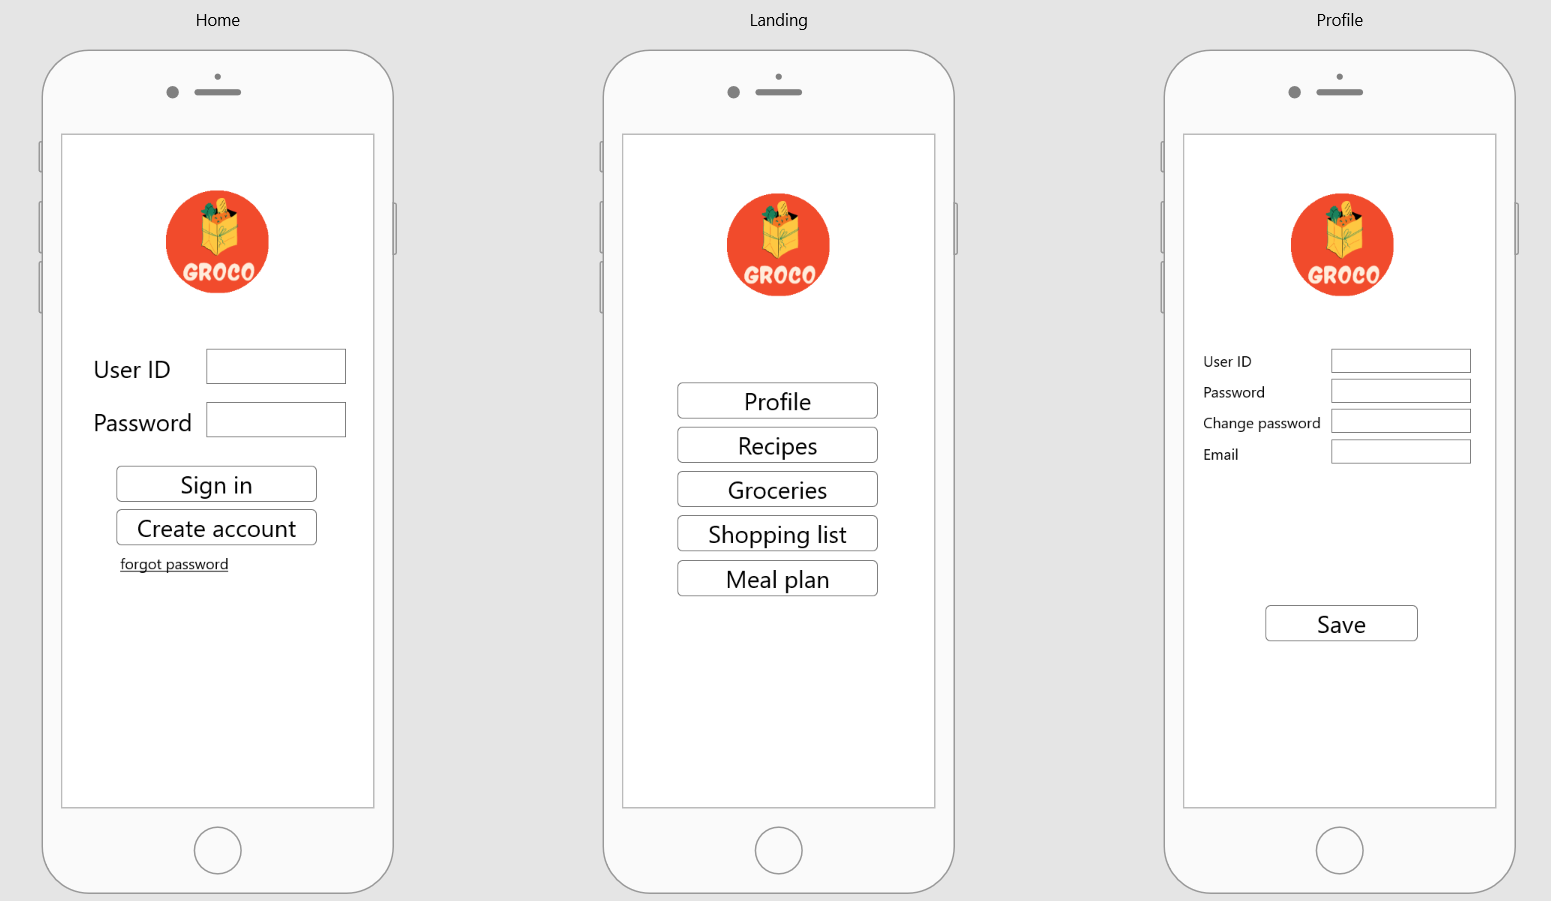
\includegraphics[width=1\textwidth]{images/I1.PNG}
   	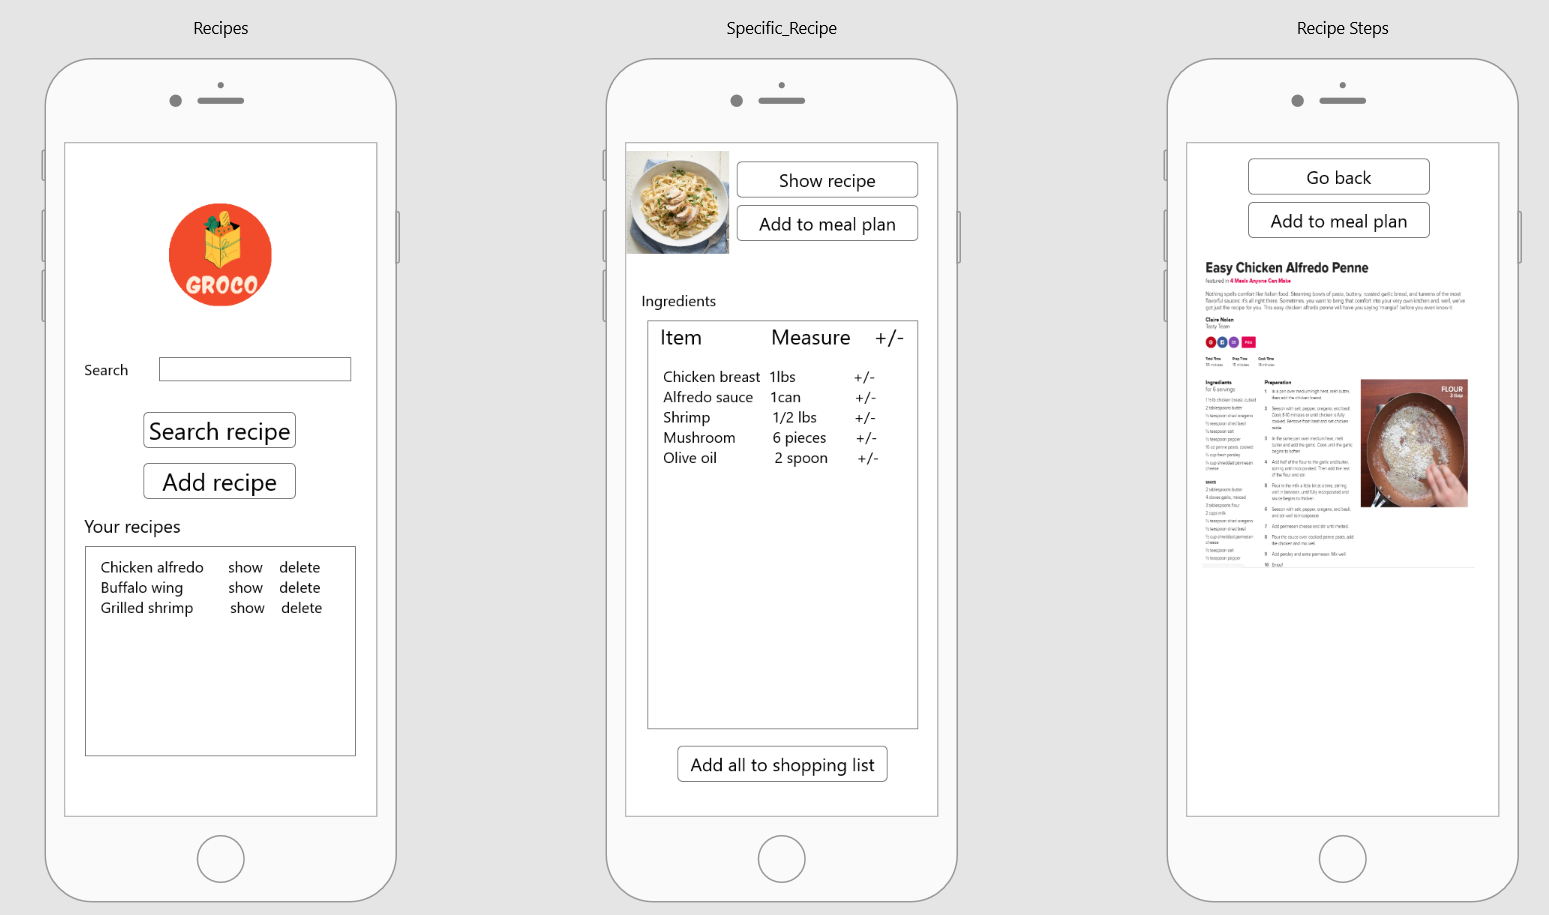
\includegraphics[width=1\textwidth]{images/I2.PNG}
\end{figure}  
\begin{figure}[H]
	\centering
   	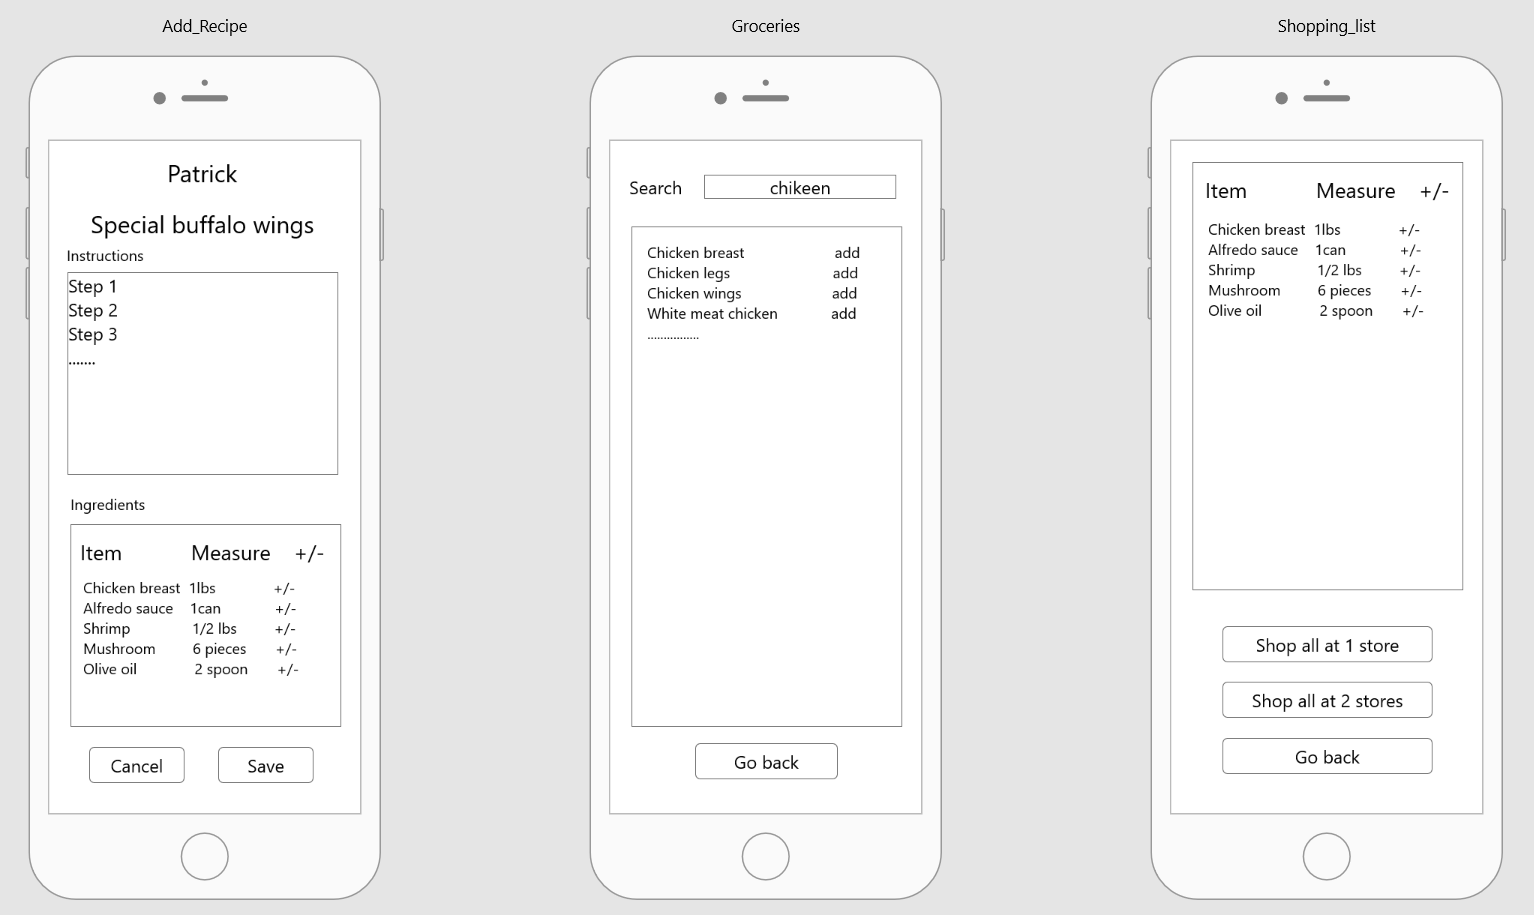
\includegraphics[width=1\textwidth]{images/I3.PNG}
   	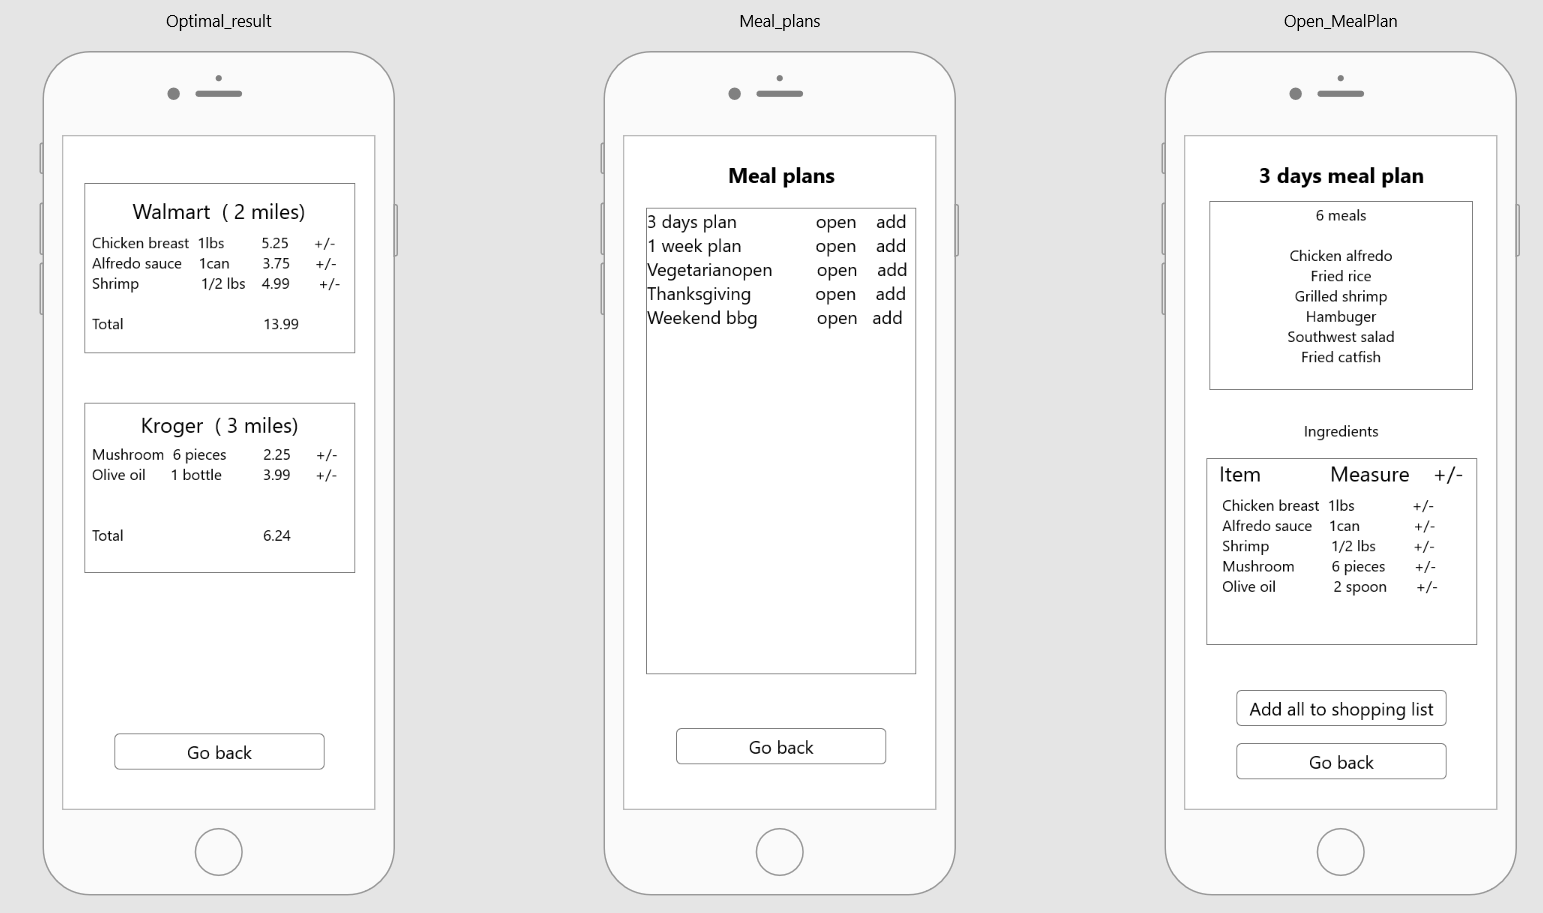
\includegraphics[width=1\textwidth]{images/I4.PNG}
   	\caption{End-user product interface}
\end{figure}  
    
    
    
    
    
    
   
   	
   	
    


\newpage
\section{Customer Requirements}
The customer requirements for this application have been procured directly from the client, Tim Dockins. The client has a good idea about end-user functionality of this application and has provided us with requirements that he thinks should be a part of the application.
\subsection{The application must allow user to search grocery items}
\subsubsection{Description}
A search functionality must be implemented into the application which will allow the user to search for a specific grocery item and then allows the user to add that item to their shopping/grocery list. The user must be allowed to type in the grocery item they are looking for and the search should find the matching item for the user to add to list.
\subsubsection{Source}
Customer
\subsubsection{Constraints}
There are chances that the search functionality may not be able to find the item that user is looking for.
\subsubsection{Priority}
High
\\
\subsection{The application must present user with the best grocery item}
\subsubsection{Description}
Based on the item that the user searched for, the application should go and look for the best possible match for that item based on the price of the item and location of the stores that item is available in. The application may list multiple options for the same item depending on the item's price and store's location.
\subsubsection{Source}
Customer
\subsubsection{Constraints}
The item searched for may not be available at any nearby store. Have to deal with the legality of web scraping from big stores.
\subsubsection{Priority}
High\\

\subsection{The application must allow users to choose references that define optimal items}
\subsubsection{Description}
The user should be able to choose brand, price, distance, and maximum stores preferences for certain grocery item.
\subsubsection{Source}
Customer
\subsubsection{Constraints}
There might be just one option available, not allowing the user to filter their search.
\subsubsection{Priority}
Moderate\\

\subsection{The application must allow users to create grocery lists}
\subsubsection{Description}
The application must allow users to create shopping lists. The shopping list must store multiple items. The user should be able to add items to their shopping list by searching for the item.
\subsubsection{Source}
Customer
\subsubsection{Constraints}
No applicable constraints.
\subsubsection{Priority}
High\\
\subsection{The application must search for all items in the shopping list}
\subsubsection{Description}
The application must search for all items in the shopping list and return the optimal items, their stores and their prices based on user specified preferences.
\subsubsection{Source}
Customer
\subsubsection{Constraints}
No applicable constraints.
\subsubsection{Priority}
High\\

\subsection{The application search for optimal items from more than one store.}
\subsubsection{Description}
When the user does a search on their entire grocery list, the application must search for the optimal results from more than one store.
\subsubsection{Source}
Customer
\subsubsection{Constraints}
The search will be limited to stores within a user specified distance.
\subsubsection{Priority}
Moderate\\

\subsection{The application must provide the most optimal route to the user}
\subsubsection{Description}
If the user opts to visit multiple stores to get their groceries then the application should provide the user with an optimal route and the order in which the user should visit those stores. The application must consider multiple factors in deciding the route. 
\subsubsection{Source}
Customer
\subsubsection{Constraints}
No applicable constraints.
\subsubsection{Priority}
Moderate\\

\subsection{The application must allow users to view and share recipes}
\subsubsection{Description}
Users should be able to look up recipes in the application. Users must also be allowed to create their own recipes and save them. The recipes will store both the ingredients for that recipe and the procedure to follow. Users must be able to view and share recipes with other users.
\subsubsection{Source}
Customer
\subsubsection{Constraints}
There must be a database available with recipes of common dishes.
\subsubsection{Priority}
Low\\

\subsection{The application must allow users to add all ingredients from a recipe to their shopping list}
\subsubsection{Description}
The application must allow the user to add all the ingredients of a recipe to their shopping list.
\subsubsection{Source}
Customer
\subsubsection{Constraints}
No applicable constraints.
\subsubsection{Priority}
Low\\

\subsection{The application must allow users to keep a list of favorite grocery items}
\subsubsection{Description}
The application must allow users to add and remove a grocery items to a favorites list. This will allow users to quickly add certain grocery items to their shopping list.
\subsubsection{Source}
Customer
\subsubsection{Constraints}
No applicable constraints.
\subsubsection{Priority}
Low

\newpage
\section{Packaging Requirements}
One of the goals is to make this application easily accessible to all users. With this in mind, the application will be presented via a web browser. This will eliminate the need for instillation files or hardware and access to certain application stores.

\subsection{Web Accessible}
\subsubsection{Description}
This product will be a web application and will be accessible to all users via web browsers on smartphones, tablets, PC, and Mac at a URL that will be specified at a later date.
\subsubsection{Source}
Customer
\subsubsection{Constraints}
Because this application will only accessible to users via web browser, an internet connection will be required.
\subsubsection{Priority}
Critical
\newpage
\section{Performance Requirements}
Include a header paragraph specific to your product here. Performance requirements address items such as: how fast specific critical operations must complete; how long it takes to start/stop activities; how long the battery must last; maximum time it must take to set up; etc.

\subsection{Grocery or Recipe Search Action}
\subsubsection{Description}
The amount of time to perform a recipe or grocery search and print out the results to the user.
\subsubsection{Source}
The Team
\subsubsection{Constraints}
Once a query is submitted, it can take no longer than four seconds.  
While the down time on the client can vary, on an average device in a cellular network it should take no more than two seconds, totalling at six seconds to complete.
In practice, caching will be an issue so it will not be uncommon for queries to take longer, but the average should be no less than six seconds.
\subsubsection{Standards}
List of applicable standards
\subsubsection{Priority}
Low

\subsection{View Recipe Menu Load Action}
\subsubsection{Description}
The amount of time required to load a recipe from a recipe query.
\subsubsection{Source}
The Team
\subsubsection{Constraints}
This action should average no more than 2 seconds and should exceed 5 seconds no more than 5\% of the time.
\subsubsection{Standards}
List of applicable standards
\subsubsection{Priority}
Low

\subsection{Add Item to List Action}
\subsubsection{Description}
The amount of time required to add an item to a shopping list.
\subsubsection{Source}
The Team
\subsubsection{Constraints}
This action should average no more than 500 milliseconds.
\subsubsection{Standards}
List of applicable standards
\subsubsection{Priority}
Low

\subsection{Compile Shopping Plan}
\subsubsection{Description}
The amount of time required to take a shopping list and choose stores and a travel route for the user.
\subsubsection{Source}
The Team
\subsubsection{Constraints}
This action should average no more than sixty seconds.
\subsubsection{Standards}
List of applicable standards
\subsubsection{Priority}
Moderate

\subsection{Load Meal Plan}
\subsubsection{Description}
The amount of time required to import a meal plan into the current shopping list.
\subsubsection{Source}
The Team
\subsubsection{Constraints}
This action should average no more than sixty seconds.
\subsubsection{Standards}
List of applicable standards
\subsubsection{Priority}
Moderate
\newpage
\section{Safety Requirements}
Due to the nature of this project, the team will only be working on software and will not need access to any labs. The team does conduct weekly meetings in the university's group study rooms and the specific policy is listed below.

\subsection{University Group Study Room Policy}
\subsubsection{Description}
All group study room users must conform to the University's policies for personal conduct: Visitor Conduct Policy. Damage to equipment in the rooms will result in the loss of the ability to reserve and/or occupy any of these rooms. Noise levels from any conversations and/or equipment must not disturb others. All group study room users are expected to be courteous and leave the room ready for the next group. Unattended personal property may not be used to "hold" a room by any individual or group and may be removed by Libraries' staff to allow others to use the space. Staff reserves the right to enter any group study room at any time. Any obstruction to the windows is prohibited. The University and its staff are not responsible for unattended, lost, stolen, or damaged personal items. \cite{UTA}
\subsubsection{Source}
University of Texas - Arlington Group Study Room Policy
\subsubsection{Constraints}
Current UTA students, faculty, and staff may reserve group study rooms with a valid UTA NetID (reserve now). A person may reserve a study room in 30-minute increments up to a maximum of 3 hours per individual per day. Reservations can be made up to 14 days in advance.
% \subsubsection{Standards}

\subsubsection{Priority}
Critical

\newpage
\section{Maintenance \& Support Requirements}
Include a header paragraph specific to your product here. Maintenance and support requirements address items specific to the ongoing maintenance and support of your product after delivery. Think of these requirements as if you were the ones who would be responsible for caring for customers/end user after the product is delivered in its final form and in use "in the field". What would you require to do this job? Specify items such as: where, how and who must be able to maintain the product to correct errors, hardware failures, etc.; required support/troubleshooting manuals/guides; availability/documentation of source code; related technical documentation that must be available for maintainers; specific/unique tools required for maintenance; specific software/environment required for maintenance; etc.

\subsection{Source Code Documentation}
\subsubsection{Description}
Detailed requirement description...
\subsubsection{Source}
Source
\subsubsection{Constraints}
Detailed description of applicable constraints...
\subsubsection{Standards}
List of applicable standards
\subsubsection{Priority}
Priority

\subsection{Amazon Web Services Maintenance}
\subsubsection{Description}
Detailed requirement description...
\subsubsection{Source}
Source
\subsubsection{Constraints}
Detailed description of applicable constraints...
\subsubsection{Standards}
List of applicable standards
\subsubsection{Priority}
Priority

\subsection{Code Commenting}
\subsubsection{Description}
Detailed requirement description...
\subsubsection{Source}
Source
\subsubsection{Constraints}
Detailed description of applicable constraints...
\subsubsection{Standards}
List of applicable standards
\subsubsection{Priority}
Priority

\newpage
\section{Other Requirements}
Include a header paragraph specific to your product here. In this section specify anything else that is required for the product to be deemed complete. Include requirements related to customer setup and configuration if not specified in a previous requirement. Add any known requirements related to product architecture/design, such as modularity, extensibility (for future enhancements), or adaptation for a specific programming language. Consider requirements such as portability of your source code to various platforms (Windows, Linux, Unix Mac OS, etc.).

\subsection{Requirement Name}
\subsubsection{Description}
Detailed requirement description...
\subsubsection{Source}
Source
\subsubsection{Constraints}
Detailed description of applicable constraints...
\subsubsection{Standards}
List of applicable standards
\subsubsection{Priority}
Priority
\newpage
\section{Future Items}
This section will cover all future requirements for this application. There is currently no plan to complete these requirements for the prototype version that will be completed for the scope of CSE 4316 and CSE 4317.

\subsection{There must be Android and iOS Applications}
\subsubsection{Description}
The prototype version, though accessible on Android and iOS devices, will only be accessible through the browser. Having applications for each type of mobile device is the highest priority of all future requirements. Having these applications will allow users to more easily access the application while creating a more efficient User Interface for mobile devices. The mobile applications should function exactly the same way on both mobile operating systems while looking as close to the same as possible, all of which should be the same as the web application.
\subsubsection{Source}
UTA STeam
\subsubsection{Constraints}
The application will have to be developed for each operating system at the same time to ensure they perform and look the same. After completion of the mobile applications, they should be made available on both the Apple App Store and Google Play Store. If any updates occur to the system, the team will have to ensure that they work and are pushed to the web, Android, and iOS applications at the same time.
% \subsubsection{Standards}
% List of applicable standards
\subsubsection{Priority}
Future

\subsection{The application must generate revenue}
\subsubsection{Description}
This application has a lot of potential to generate revenue. The two main ways this can be done would be through data collection or membership access. Data collection could be useful to companies that want to track what certain demographics are shopping for, which zip codes people are shopping in, or how far people are will to drive for certain stores, etc. Memberships could allow for partnerships with other companies. This could allow certain people or companies to release cookbooks in the application, dietitians to create personalized meal plans for users, or allow stores to offer exclusive deals all of which would only be accessible to members.
\subsubsection{Source}
Customer
\subsubsection{Constraints}
The stakeholders must come to an agreement on how the application will generate revenue. If data collection is decided upon, the development team must ensure that all laws and regulations are followed and allow users to opt out of collection. If membership is chosen, the stakeholders must find partners that could make a membership worth the user's money.
% \subsubsection{Standards}
% List of applicable standards
\subsubsection{Priority}
Future

\subsection{The application must allow users to rate recipes}
\subsubsection{Description}
Users will have the ability to rate recipes. The rating system will be a standard five-star system. This rating system will allow users to make the best choice when looking at similar recipes.
\subsubsection{Source}
UTA STeam
\subsubsection{Constraints}
The development team will have to find a way to prevent users from spamming recipes with five-star ratings to boost traffic to a recipe. There will also need to be a way to prevent users from spamming a recipe with bad reviews for illegitimate reasons.
% \subsubsection{Standards}
% List of applicable standards
\subsubsection{Priority}
Future

\subsection{The application must allow users to review recipes}
\subsubsection{Description}
The review system will allow user to give any general comments about the recipe. This will also allow users to share their critiques, helpful tips, and recommendations. 
\subsubsection{Source}
UTA STeam
\subsubsection{Constraints}
There will have to be a way to regulate these comments to ensure that nothing offensive is said in the reviews. There should also be a way to ensure that these reviews are only relevant to the recipe.
% \subsubsection{Standards}
% List of applicable standards
\subsubsection{Priority}
Future

\subsection{The application must allow users to report recipes}
\subsubsection{Description}
The recipe reporting system will allow users to report recipes. Once they are reported, someone within the team should be tasked with screening these reports to ensure their legitimacy. This reporting system will help the team ensure that shared recipes are in fact recipes, that recipes do not contain or create anything harmful or illegal, while also regulating any vulgar or offensive language that might appear in the recipes.
\subsubsection{Source}
UTA STeam
\subsubsection{Constraints}
The team will have to regulate reporting to ensure that they are legitimate.
% \subsubsection{Standards}
% List of applicable standards
\subsubsection{Priority}
Future

\subsection{The application will have an enhanced search algorithm}
\subsubsection{Description}
The algorithm for the prototype version of this application  will provide the most optimal grocery item based only on price and location. In the future, customers will be able to choose the criteria that chooses the optimal grocery item. This will allow users to give their own priority to brand, price, or location. The user will give a list of weights to each priority and the algorithm will prioritize based on those weights to give the optimal locations, items, and path.
\subsubsection{Source}
Customer
\subsubsection{Constraints}
The team will have to create an algorithm that is able to change based on user preference.
% \subsubsection{Standards}
% List of applicable standards
\subsubsection{Priority}
Future
\newpage

%%% References
\bibliographystyle{plain}
\bibliographystyle{reference/IEEEtran_custom}
\bibliography{reference/refs}{}

\end{document}